%----------------------------------------------------------------------------------------
%	CHAPTER - SUGGESTION
%----------------------------------------------------------------------------------------

\chapter{Suggestion}

\label{ChapterSuggestion}

%----------------------------------------------------------------------------------------
%	SECTION 1
%----------------------------------------------------------------------------------------

\section{Introduction}

The in chapter \ref{DSRCycle} discussed \gls{dsr} cycle from \cite{Vaishnavi2008} and \cite{Hevner2010} defines \textit{Suggestion} as the next step after \textit{Awareness of Problem}. \cite{Vaishnavi2008} define the \textit{Suggestion} phase as a creative step in which new functionality is envisioned to form a tentative design for the development of the prototype. \cite{Vaishnavi2008} further specifies the output as a constructed theory that addresses the identified problem, which can include new ideas and concepts, new methods, and new models that in the end shall be validated with the development of the prototype. \newline
In a first step, the end goals of the design are defined which will be relevant for the evaluation in chapter \ref{ChapterEvaluation}. Then the individual views of presentation (e.g. an overview and detail view) are defined as well as the navigation between them. As the third step, the visualisation of the individual views are defined before finally the interaction patterns (action/reaction) can be mapped to them. Building up on this, the \textit{Development} phase will then be discussed in chapter \ref{ChapterDevelopment}.


%----------------------------------------------------------------------------------------
%	SECTION 2
%----------------------------------------------------------------------------------------

\section{Goals of the Design}

In order to define the goals of the design, the specific characteristics of \gls{vr} itself and the to be visualised data have to be considered. In this thesis, the goals are defined either as \glspl{mdg} for the more overarching goals, or as \glspl{sdg} which are focussing rather on specific areas. In the following sub-chapters, these characteristics are discussed in more detail and the individual goals are defined over the three main categories: \gls{vr}, data, and visualisation.
\newcounter{MainDesignGoalCounter} % Create two new counters
\newcounter{SubDesignGoalCounter}
\stepcounter{MainDesignGoalCounter} % Increas both values from 0 to 1
\stepcounter{SubDesignGoalCounter}

%-----------------------------------
%	SUBSECTION 1
%-----------------------------------
\subsection{\gls{vr}-specific Goals}

The goals that are derived from \gls{vr} itself, are more high-level since they can be applied to any \gls{vr} application independent of what its purpose is. Therefore, the three important characteristics of \gls{vr} as defined by \cite{Stone1994} and discussed in chapter \ref{SubSectionVisualisationManipulation} are considered as an integral part of the design. These characteristics can be summarized in the following three keywords: Action/Reaction, Immersion and Spatial. Based on these, the first \glspl{mdg} from a \gls{vr} perspective can be derived and further described with examples:
\begin{itemize}[noitemsep,nolistsep]
	\item \textbf{\gls{mdg} \arabic{MainDesignGoalCounter}:} High interactivity with tightly coupled actions/reactions \newline
		\textit{Example: No slow animations, no timed events, or any other change in scenery without a trigger from the user}
		\stepcounter{MainDesignGoalCounter}
	\item \textbf{\gls{mdg} \arabic{MainDesignGoalCounter}:} The user is part of the \gls{ve} and thus is able to 'travel' around the visualisations \newline
		\textit{Example: Movement at free will, and no outside view, or third-person \gls{pov}}
		\stepcounter{MainDesignGoalCounter}
	\item \textbf{\gls{mdg} \arabic{MainDesignGoalCounter}:} The design is intended for \gls{vr} and thus in full 3D \newline
		\textit{Example: No flattened two-dimensional representation in 3D space}
		\stepcounter{MainDesignGoalCounter}
\end{itemize}
In addition to the above characteristics, another goal has to be that the design should not rely on specific \gls{vr}-hardware, but rather define them in a more abstract way as to what the individual hardware items should be capable of. Since this topic is only important for the \gls{vr} input devices and potentially the \gls{hmd} but not the visualisation itself, it is considered as a \gls{sdg}.
\begin{itemize}[noitemsep,nolistsep]
	\item \textbf{\gls{sdg} \arabic{SubDesignGoalCounter}:} The design is independent of specific \gls{vr} hardware \newline
		\textit{Example: No direct references to specific hardware, but rather what the hardware has to be capable of (requirements)}
		\stepcounter{SubDesignGoalCounter}
\end{itemize}
From a \gls{vr} perspective, the important areas can all be covered with the above defined goals. The main aspects of the design are depending on what data is used and thus is discussed in the following sub-chapter.


%-----------------------------------
%	SUBSECTION 2
%-----------------------------------

\subsection{Data-specific Goals}

The data set that is used for this thesis is shown in Appendix \ref{AppendixA} and contains information about categorized financial expenses of one year. The focus for the data-specific goals is put on this specific data-set and might only partially be applicable to other data sets. Since the goal of this thesis is to enhance the current interaction with the data, the presentation should provide \textbf{at least} the same amount of information to the user.
\begin{itemize}[noitemsep,nolistsep]
	\item \textbf{\gls{mdg} \arabic{MainDesignGoalCounter}:} The design provides at least the same information as  existing applications \newline
		\textit{Example: View on individual months or the whole year, summed-up expenses based on their category, or easy comparison of different categories (based on total amount)}
		\stepcounter{MainDesignGoalCounter}
\end{itemize}
In order to provided an added value to the user, further quality of life features such as direct access to the underlying transactions, the filtering of individual categories, or the display of a (spending) trend are considered. They support the main functionality of data exploration by rendering certain tasks easier and more convenient for the user. Due to this supporting aspect, this is considered as a \gls{sdg}.
\begin{itemize}[noitemsep,nolistsep]
	\item \textbf{\gls{sdg} \arabic{SubDesignGoalCounter}:} The design includes new quality-of-life features \newline
	\textit{Example: Direct access to underlying transactions, filtering of individual (sub-)categories, or the display of a (spending) trend-line}
	\stepcounter{SubDesignGoalCounter}
\end{itemize}


%-----------------------------------
%	SUBSECTION 3
%-----------------------------------

\subsection{Visualisation Goals}

The \gls{vism} from \cite{Shneiderman2005} (see chapter \ref{SubSectionVISM}) has proven to be a solid base design principle whenever the to be executed work is focussed on finding information. This matches the situation of analysing ones financial expenses very well and thus is seen as one of the \gls{mdg} from a visualisation perspective.
\begin{itemize}[noitemsep,nolistsep]
	\item \textbf{\gls{mdg} \arabic{MainDesignGoalCounter}:} The design follows the \gls{vism} \newline
		\textit{Overview first, zoom and filter, then details-on-demand}
		\stepcounter{MainDesignGoalCounter}
\end{itemize}
In addition, the design should also include the improvements from \gls{vism} 2.0 by adhering to the seven main tasks as defined by \cite{Stauffer2016} and shown in Figure \ref{fig:vism2}. The three support tasks (i.e. History, Extract, and Collaboration) are not considered to be relevant for the prototype since they are only support tasks and thus not relevant for the main functionality. They however could become relevant for future research in this area. Since version 2.0 is an enhancement to the existing mantra, it is deemed as a \gls{sdg}.
\begin{itemize}[noitemsep,nolistsep]
	\item \textbf{\gls{sdg} \arabic{SubDesignGoalCounter}:} The design adheres to the seven main tasks of \gls{vism} 2.0 \newline
		\textit{Main Tasks: Overview, Zoom In, Zoom Out, Filtering, Relate, Details, and Multi View}
		\stepcounter{SubDesignGoalCounter}
\end{itemize}

% For the "conclusion", we have to remove "1" from the counter again:
\addtocounter{MainDesignGoalCounter}{-1}
\addtocounter{SubDesignGoalCounter}{-1}
% -------------------------------------------
With this, all goals that are relevant for the design have been covered and summarized into \arabic{MainDesignGoalCounter} \glspl{mdg} and \arabic{SubDesignGoalCounter} \glspl{sdg}. The next chapter focuses on the definition of the individual views that are available, and how the navigation in between them is defined.


%----------------------------------------------------------------------------------------
%	SECTION 3
%----------------------------------------------------------------------------------------

\section{View Definition and Navigation Map}

\newcounter{ViewCounter} % Create a new counter
\stepcounter{ViewCounter} % Increase value from 0 to 1

In a first step, the different individual views are defined, before a navigation map can be defined that shows what transitions can be possible from one view to another.


%-----------------------------------
%	SUBSECTION 1
%-----------------------------------

\subsection{View Definition}

\cite{Shneiderman1996} defined the following mantra as the fundamental visual design guideline:
\begin{framed}
	\textit{Overview first, zoom and filter, then details-on-demand}
\end{framed}
This mantra already clearly distinguishes between to main views: overview and detail. By looking at the \textit{Overview} perspective in regards to the financial expenses, this either could be a summary of the current year, or a bit more detailed the summary of the current month, or even just a 'blank page' where the first entry point has to be chosen from. The last interpretation goes in the direction of what \cite{Neil2006} claimed to be one of the big downfalls of \gls{vism}, that a user might already know what data he wants to see and thus does not want to start on an overview and then dig down to the details. Due to the increased available space in \gls{vr}, it however becomes possible to fulfil all of these demands by presenting all three options next to each other. This also relates to the idea of the \textit{Multi View} which is one of the seven main tasks of \gls{vism} 2.0 as defined by \cite{Stauffer2016}. This allows to define the first three views:
\begin{itemize}[noitemsep,nolistsep]
	\item \textbf{View \arabic{ViewCounter}:} Overview of (current) year
	\stepcounter{ViewCounter}
	\item \textbf{View \arabic{ViewCounter}:} Overview of (current) month
	\stepcounter{ViewCounter}
	\item \textbf{View \arabic{ViewCounter}:} Selection of different month/year
	\stepcounter{ViewCounter}
\end{itemize}
The next main task from \gls{vism} 2.0 which is also part of the original mantra is about \textit{Filtering}, which in this (data) context can be applied to the different main and subcategories as shown in Table \ref{tbl:financialcategories} in Chapter \ref{ChapterIntroduction}. To further adhere to the \textit{Multi View} task, the filtering is put in an additional view to not interfere with the actual data visualisation.
\begin{itemize}[noitemsep,nolistsep]
	\item \textbf{View \arabic{ViewCounter}:} Filtering of main and subcategories
	\stepcounter{ViewCounter}
\end{itemize}
Continuing the main tasks from \gls{vism} 2.0, we come to \textit{Details} which for the data set that is used in this thesis is a single individual financial transaction. This additional view provides all detailed information about the transaction, from date over amount and recipient to the categories. Since it however is not directly possible to go from a grouped view into a single transaction, an intermediate view that lists all transactions has to be added.
\begin{itemize}[noitemsep,nolistsep]
	\item \textbf{View \arabic{ViewCounter}:} Overview of filtered financial transactions
	\stepcounter{ViewCounter}
	\item \textbf{View \arabic{ViewCounter}:} Details of a single financial transaction
	\stepcounter{ViewCounter}
\end{itemize}


% For the "conclusion", we have to remove "1" from the counter again:
\addtocounter{ViewCounter}{-1}
% -------------------------------------------
This concludes all the relevant views for the design. In the next step, the navigation between them are defined which covers the \textit{Relate}, \textit{Zoom In} and \textit{Zoom Out} tasks from the \gls{vism} 2.0.


%-----------------------------------
%	SUBSECTION 2
%-----------------------------------

\subsection{Navigation Map}

After the definition of all views, the navigation in between them has to be defined. The base principle for the definition is again the \gls{vism} to make sure it is possible to navigate from the overview into the detail view. Figure \ref{fig:navigationmap} shows the proposed navigation map with all previously defined views. The four green views (1, 2, 5, and 6) are considered the main views where actual data is presented, whereas the two blue views (3 and 4) are considered the supporting views that do not display any actual data, but rather help with the navigation between the main screens. The green arrows indicate the main navigation flow, whereas the orange ones can provide shortcuts directly from the main views themselves. \newline
\begin{figure}[h]
	\begin{center}
		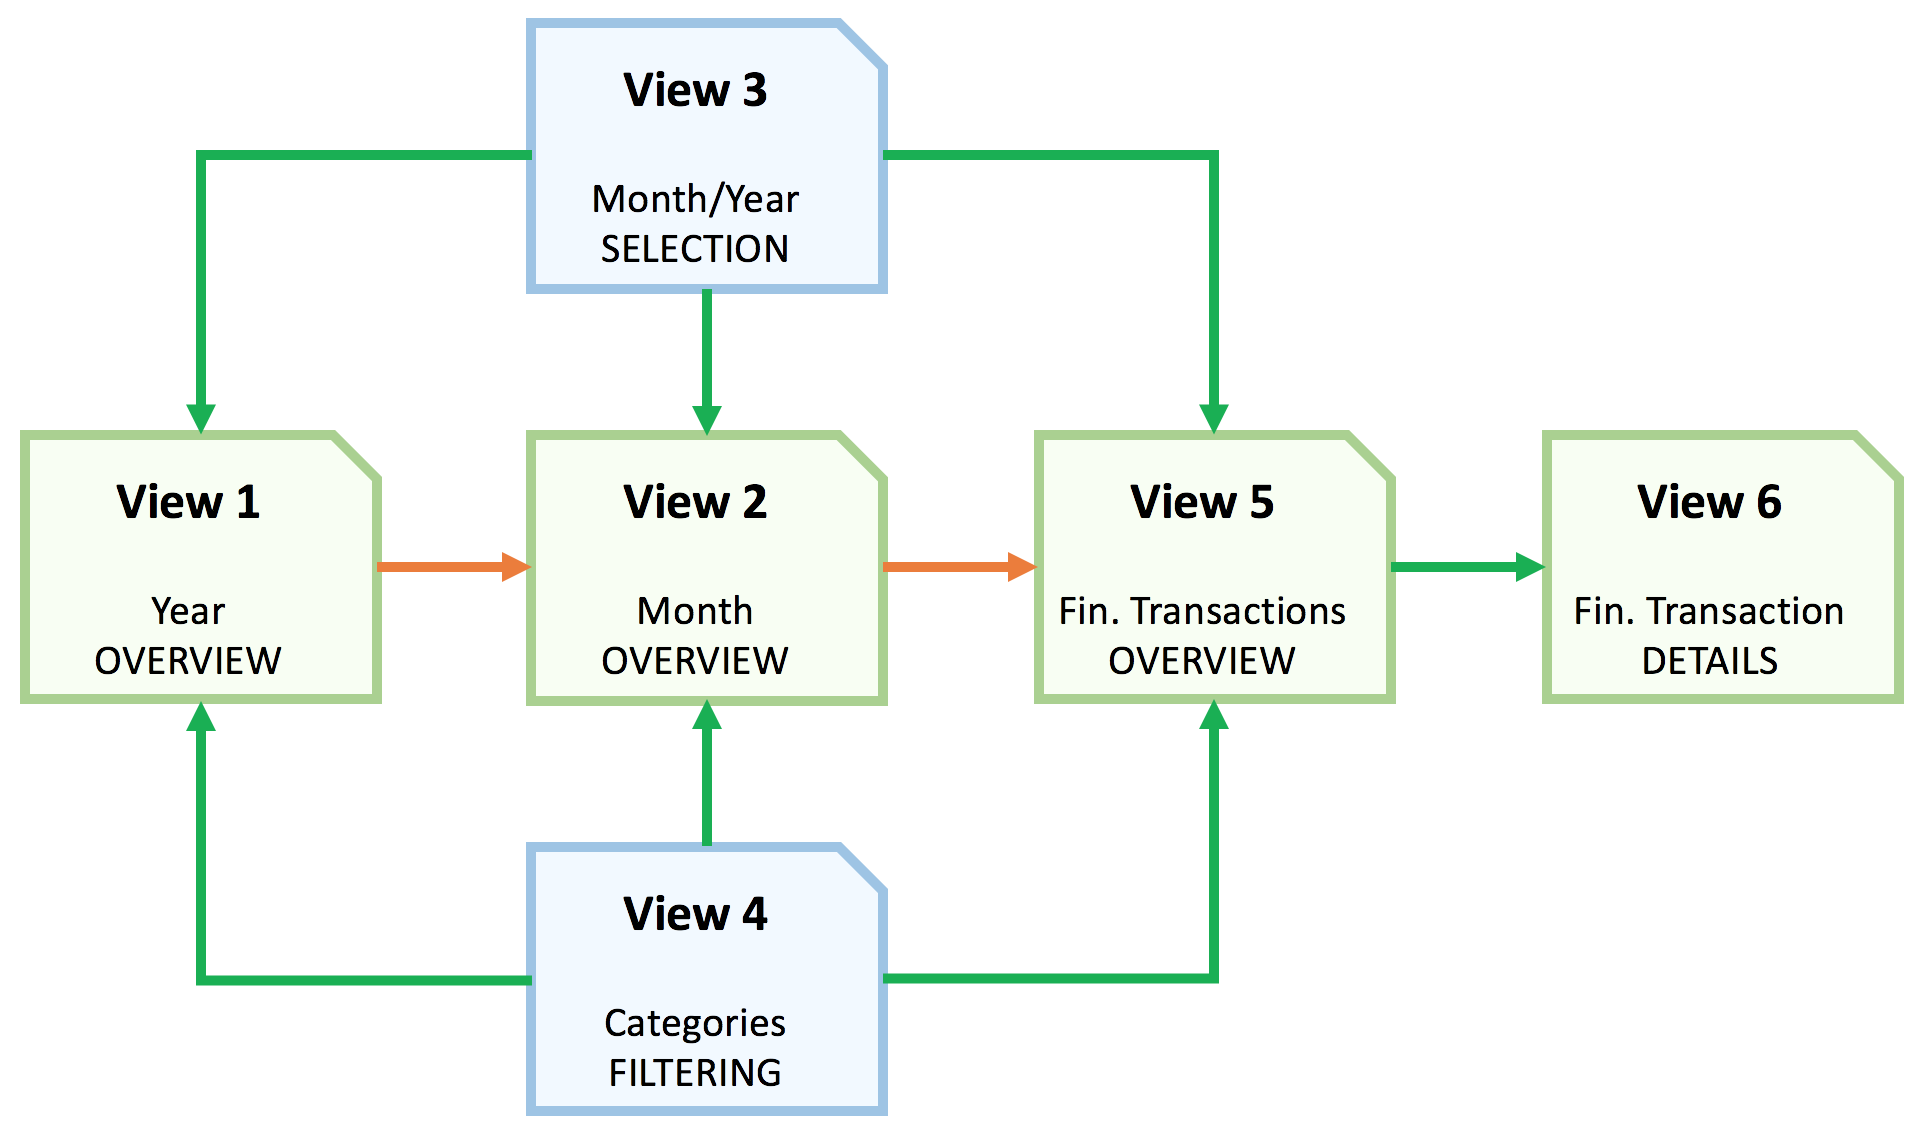
\includegraphics[width=14cm]{03_Figures/07_Suggestion/NavigationMap.png}
		\caption{Navigation Map of Design Suggestion}
		\label{fig:navigationmap}
	\end{center}
\end{figure}

For a better understanding, in Table \ref{tbl:navigationmap} each navigation flow is explained in more detail.
\begin{longtable}{ | p{2.5cm} | p{11.5cm} |}
	\hline
	\textbf{Flow} & \textbf{Description} \\
	\hline
	\endfirsthead % Line(s) to appear as head of the table on the first page
	\multicolumn{2}{c}%
	{\tablename\ \thetable\ -- \textit{Continued from previous page}} \\
	\hline
	\textbf{Flow} & \textbf{Description} \\
	\hline
	\endhead % Line(s) to appear at top of every page (except first)
	\hline
	\multicolumn{2}{r}{\textit{Continued on next page}} \\
	\endfoot % Last line(s) to appear at the bottom of every page (except last)
	\endlastfoot % Last line(s) to appear at the end of the table
	\hline
	View 1 \textrightarrow{} 2 &
	\textbf{From} Year OVERVIEW \textbf{to} Month OVERVIEW \newline
	This supporting flow allows the selection of a specific month, directly from the display of the year overview and thus can be seen as shortcut over view 3. \\
	\hline
	View 2 \textrightarrow{} 5 &
	\textbf{From} Month OVERVIEW \textbf{to} Fin. Transactions OVERVIEW \newline
	The second supporting flow enables the selection of an individual day, directly from the display of the month to apply an additional filter on view 5. \\
	\hline
	View 3 \textrightarrow{} 1 &
	\textbf{From} Month/Year SELECTION \textbf{to} Year OVERVIEW \newline
	tbd \\
	\hline
	View 3 \textrightarrow{} 2 &
	\textbf{From} Month/Year SELECTION \textbf{to} Month OVERVIEW \newline
	tbd \\
	\hline
	View 3 \textrightarrow{} 5 &
	\textbf{From} Month/Year SELECTION \textbf{to} Fin. Transactions OVERVIEW \newline
	tbd \\
	\hline
	View 4 \textrightarrow{} 1 &
	\textbf{From} Categories FILTERING \textbf{to} Year OVERVIEW \newline
	tbd \\
	\hline
	View 4 \textrightarrow{} 2 &
	\textbf{From} Categories FILTERING \textbf{to} Month OVERVIEW \newline
	tbd \\
	\hline
	View 4 \textrightarrow{} 5 &
	\textbf{From} Categories FILTERING \textbf{to} Fin. Transactions OVERVIEW \newline
	tbd \\
	\hline
	View 5 \textrightarrow{} 6 &
	\textbf{From} Fin. Transactions OVERVIEW \textbf{to} Fin. Transaction DETAIL \newline
	tbd \\
	\hline
	\caption{Explanation of the different flows in the navigation map}
	\label{tbl:navigationmap}
\end{longtable}






Relate (view relationships)

Details

Zoom In/Out

- Navigation Map / "Screen-Flow"



%----------------------------------------------------------------------------------------
%	SECTION 4
%----------------------------------------------------------------------------------------

\section{Visualisation of Views and Data}

- Exact Presentation of Data (how look like?)


%----------------------------------------------------------------------------------------
%	SECTION 5
%----------------------------------------------------------------------------------------

\section{Mapping of Interaction Patterns}

- Action/Reaction (Interaction)




%----------------------------------------------------------------------------------------
%	SECTION 6
%----------------------------------------------------------------------------------------

\section{Conclusion}



%% IDEA FOR PROTOTYPE

- Start with a small table on which a house etc is visualized. floating above is year (+month)
- Each object represents one category from the financial expenses.
- maybe size indicates the overall amount?
- The colours depends on the difference between my planned expenses (or average expenses) and the actual expenses. less = green, about the same = yellow-(green-)ish, slightly above = orange, above = red.
- By clicking on one of the objects, it gets highlighted and a line-chart appears showing the expenses
   A) show individual transactions for the given month up until the threshold
   B) show individual months until the threshold (+forecast?)
- show multiple lines for the different sub-categories (enable/disable) plus the total
- clicking on an entry of the line chart displays details about transaction (amount, location), or the month (amount) in an overlay
- switching between single-month and year view by... using the touchpad (up/down clicks)
- navigating through months/years by... a using the touchpad! (left/right clicks)
- resetting the view to start by... clicking on the select button

- maybe outside as rotating rings: the individual bank accounts?

